%%%%%%%%%%%%%%%%%%%%%%%%%%%%%%%%%%%%%%%%%%%%%%%%%%%%%%%%%%%%%%%%%%%%%
%% This is a (brief) model paper using the achemso class
%% The document class accepts keyval options, which should include
%% the target journal and optionally the manuscript type. 
%%%%%%%%%%%%%%%%%%%%%%%%%%%%%%%%%%%%%%%%%%%%%%%%%%%%%%%%%%%%%%%%%%%%%
\documentclass[journal=jacsat,manuscript=article]{achemso}
\usepackage{multicol}
\usepackage{graphicx}% Include figure files
\usepackage{graphicx}% Include figure files
\usepackage{dcolumn}% Align table columns on decimal point
\usepackage{bm}% bold math
%\usepackage[mathlines]{lineno}% Enable numbering of text and display math
%\linenumbers\relax % Commence numbering lines
\usepackage{pgffor}
\usepackage[utf8]{inputenc}
\usepackage[T1]{fontenc}
\usepackage{mathptmx}
\usepackage{listings}
\lstset{language=Python}
\usepackage{rotating} % Rotating table
\usepackage{caption}
\usepackage{subcaption}

\usepackage{color}
\usepackage{dcolumn} % decimal align in tables
\usepackage{bm} % bold math
\usepackage{graphicx}
\usepackage{multirow} % for table cells to span rows
\usepackage{pifont} % for checkmarks
\usepackage{epsfig}
\usepackage{amsmath} % matrix
% \usepackage{subfigure}
\usepackage{float}
\usepackage{booktabs}
\usepackage{tabularx}
\usepackage{natbib}
\usepackage{gensymb}
\setlength{\paperwidth}{8.5in}
\setlength{\paperheight}{11.0in}
\usepackage{rotating}
\usepackage{threeparttable}
\usepackage{comment}
%for corrections
\usepackage[normalem]{ulem}
% \usepackage{xr-hyper}
\usepackage[hidelinks]{hyperref} % allows hyperlinking for references
%%%%%%%%%%%%%%%%%%%%%%%%%%%%%%%%%%%%%%%%%%%%%%%%%%%%%%%%%%%%%%%%%%%%%
%% Place any additional packages needed here.  Only include packages
%% which are essential, to avoid problems later. Do NOT use any
%% packages which require e-TeX (for example etoolbox): the e-TeX
%% extensions are not currently available on the ACS conversion
%% servers.
%%%%%%%%%%%%%%%%%%%%%%%%%%%%%%%%%%%%%%%%%%%%%%%%%%%%%%%%%%%%%%%%%%%%%
\usepackage[version=3]{mhchem} % Formula subscripts using \ce{}
\usepackage{xcolor}
% \usepackage{xr-hyper}
\usepackage{xr-hyper}
\usepackage{xr}


\usepackage[hidelinks]{hyperref} % allows hyperlinking for references

% \usepackage{hyperref}
\usepackage{amsmath,amssymb,amsthm}
\usepackage{mathtools,physics}


\usepackage{subcaption}
\usepackage{caption}
% \usepackage{titling}
%%%%%%%%%%%%%%%%%%%%%%%%%%%%%%%%%%%%%%%%%%%%%%%%%%%%%%%%%%%%%%%%%%%%%
%% If issues arise when submitting your manuscript, you may want to
%% un-comment the next line.  This provides information on the
%% version of every file you have used.
%%%%%%%%%%%%%%%%%%%%%%%%%%%%%%%%%%%%%%%%%%%%%%%%%%%%%%%%%%%%%%%%%%%%%
%%\listfiles

%%%%%%%%%%%%%%%%%%%%%%%%%%%%%%%%%%%%%%%%%%%%%%%%%%%%%%%%%%%%%%%%%%%%%
%% Place any additional macros here.  Please use \newcommand* where
%% possible, and avoid layout-changing macros (which are not used
%% when typesetting).
%%%%%%%%%%%%%%%%%%%%%%%%%%%%%%%%%%%%%%%%%%%%%%%%%%%%%%%%%%%%%%%%%%%%%
\newtheorem{theorem}{Theorem}[section]
\newtheorem{corollary}{Corollary}
\newtheorem{lemma}[theorem]{Lemma}
\newtheorem{proposition}{Proposition}
\newtheorem{conjecture}{Conjecture}
\newtheorem{definition}[theorem]{Definition}
\newtheorem{assumption}[theorem]{Assumption}
% \newtheorem{example}[theorem]{Example}
\newtheorem{example}{Example}[section]
\newtheorem{remark}{Remark}

% Add line numbers, as requested by Nature
\usepackage{lineno}
% \linenumbers


\newcommand*\mycommand[1]{\texttt{\emph{#1}}}
\newcommand{\noteg}[1]{\textcolor{red}{({Grier: #1})}}
\newcommand{\notek}[1]{\textcolor{darkspringgreen}{({Kostas: #1})}}


%%%% HELPER CODE FOR DEALING WITH EXTERNAL REFERENCES
% (from an answer by cyberSingularity at http://tex.stackexchange.com/a/69832/226)
%%%

\usepackage{xcite}

%%%%%%%%%%%%%%%%%%%%%%%%%%%%%%%%%%%%%%%%%%%%%%%%%%%%%%%%%%%%%%%%%%%%%%%%
%----Helper code for dealing with external references----
% (by cyberSingularity at http://tex.stackexchange.com/a/69832/226)

\usepackage{xr}
\makeatletter

\newcommand*{\addFileDependency}[1]{% argument=file name and extension
\typeout{(#1)}% latexmk will find this if $recorder=0
% however, in that case, it will ignore #1 if it is a .aux or 
% .pdf file etc and it exists! If it doesn't exist, it will appear 
% in the list of dependents regardless)
%
% Write the following if you want it to appear in \listfiles 
% --- although not really necessary and latexmk doesn't use this
%
\@addtofilelist{#1}
%
% latexmk will find this message if #1 doesn't exist (yet)
\IfFileExists{#1}{}{\typeout{No file #1.}}
}\makeatother

\newcommand*{\myexternaldocument}[1]{%
\externaldocument{#1}%
\addFileDependency{#1.tex}%
\addFileDependency{#1.aux}%
}
%------------End of helper code--------------

% put all the external documents here!
\myexternaldocument{SI}
\newcommand{\siref}[1]{\ref{#1}}
%%%%%%%%%%%%%%%%%%%%%%%%%%%%%%%%%%%%%%%%%%%%%%%%%%%%%%%%%%%%%%%%%%%%%%%%


%%%%%%%%%%%%%%%%%%%%%%%%%%%%%%%%%%%%%%%%%%%%%%%%%%%%%%%%%%%%%%%%%%%%%
%% The document title should be given as usual. Some journals require
%% a running title from the author: this should be supplied as an
%% optional argument to \title.
%%%%%%%%%%%%%%%%%%%%%%%%%%%%%%%%%%%%%%%%%%%%%%%%%%%%%%%%%%%%%%%%%%%%%
\title{A Combinatorial Search of Parameterized Quantum Circuit Learning for Chemical Applications}
%%%%%%%%%%%%%%%%%%%%%%%%%%%%%%%%%%%%%%%%%%%%%%%%%%%%%%%%%%%%%%%%%%%%%
%% Meta-data block
%% ---------------
%% Each author should be given as a separate \author command.
%%
%% Corresponding authors should have an e-mail given after the author
%% name as an \email command. Phone and fax numbers can be given
%% using \phone and \fax, respectively; this information is optional.
%%
%% The affiliation of authors is given after the authors; each
%% \affiliation command applies to all preceding authors not already
%% assigned an affiliation.
%%
%% The affiliation takes an option argument for the short name.  This
%% will typically be something like "University of Somewhere".
%%
%% The \altaffiliation macro should be used for new address, etc.
%% On the other hand, \alsoaffiliation is used on a per author basis
%% when authors are associated with multiple institutions.
%%%%%%%%%%%%%%%%%%%%%%%%%%%%%%%%%%%%%%%%%%%%%%%%%%%%%%%%%%%%%%%%%%%%%
\author{Grier M. Jones}
\affiliation[UTSG ECE]{
The Edward S. Rogers Sr. Department of Electrical and Computer Engineering, 
University of Toronto, 
10 Kings College Road, Toronto, Ontario, 
Canada M5S 3G4}
\alsoaffiliation[UTM CHEM]{
Department of Chemical and Physical Sciences, 
University of Toronto Mississauga, 
3359 Mississauga Road, Mississauga, Ontario, 
Canada L5L 1C6}

\author{Nick Taylor}
\affiliation[UTSG ECE]{
The Edward S. Rogers Sr. Department of Electrical and Computer Engineering, 
University of Toronto, 
10 Kings College Road, Toronto, Ontario, 
Canada M5S 3G4}
          
\author{Viki Kumar Prasad}
\affiliation[UTSG ECE]{
The Edward S. Rogers Sr. Department of Electrical and Computer Engineering, 
University of Toronto, 
10 Kings College Road, Toronto, Ontario, 
Canada M5S 3G4}
\alsoaffiliation[UTM CHEM]{
Department of Chemical and Physical Sciences, 
University of Toronto Mississauga, 
3359 Mississauga Road, Mississauga, Ontario, 
Canada L5L 1C6}



\author{Ulrich Fekl}
\affiliation[UTM CHEM]{
Department of Chemical and Physical Sciences, 
University of Toronto Mississauga, 
3359 Mississauga Road, Mississauga, Ontario, 
Canada L5L 1C6}
\email{ulrich.fekl@utoronto.ca}

\author{Hans-Arno Jacobsen}
\affiliation[UTSG ECE]{
The Edward S. Rogers Sr. Department of Electrical and Computer Engineering, 
University of Toronto, 
10 Kings College Road, Toronto, Ontario, 
Canada M5S 3G4}
\email{jacobsen@eecg.toronto.edu}
%%%%%%%%%%%%%%%%%%%%%%%%%%%%%%%%%%%%%%%%%%%%%%%%%%%%%%%%%%%%%%%%%%%%%
%% Some journals require a list of abbreviations or keywords to be
%% supplied. These should be set up here, and will be printed after
%% the title and author information, if needed.
%%%%%%%%%%%%%%%%%%%%%%%%%%%%%%%%%%%%%%%%%%%%%%%%%%%%%%%%%%%%%%%%%%%%%
\abbreviations{}
\keywords{American Chemical Society, \LaTeX}

%%%%%%%%%%%%%%%%%%%%%%%%%%%%%%%%%%%%%%%%%%%%%%%%%%%%%%%%%%%%%%%%%%%%%
%% The manuscript does not need to include \maketitle, which is
%% executed automatically.
%%%%%%%%%%%%%%%%%%%%%%%%%%%%%%%%%%%%%%%%%%%%%%%%%%%%%%%%%%%%%%%%%%%%%
\newcommand{\R}{\mathbb{R}}

\begin{document}

\section{Abstract}
The rapid growth of quantum computing has seen a rise in the development of applicable near-term quantum algorithms. A promising candidate to run on current noisy intermediate-scale quantum (NISQ) hardware is quantum machine learning (QML). Parameterized quantum circuits can be learned as models in a hybrid classical-quantum approach. It has been shown that QML models may need less training data to generalize compared to classical methods. Although QML has been explored largely within classification tasks, regression tasks have received much less attention. Existing studies have only utilized few qubits and lack relevant practical applications. We will discuss our work on the development and comparisons of QML models for highly desired prediction of chemical properties such as bond dissociation energies and barrier height energies. Our work investigates the trainability, expressibility, and generalization capability of various quantum models for the purpose of regression of molecular properties. Our work also provides a benchmark against classical machine learning models and implications of using error mitigation techniques for QML. \par

\newpage
\begin{itemize}
	\item Abstract
	\item Introduction
	\item Methods
	\item Datasets
	\item Results and Discussion
	\begin{itemize}
		\item Function fitting 
		\begin{itemize}
			\item All (5 + 16 qubit)
			\item RUD + AL (5 + 16 qubit)
			\item Error mitigation on FakeQuebec
		\end{itemize}
		\item BSE
		\begin{itemize}
			\item All 5 qubit
			\item Truncated 16 qubit set (cost analysis 5 qubit)
			\item RUD + AL (5 + 16 qubit)
			\item Real device (without error mitigation and with whatever the best is from function fitting)
		\end{itemize}		
		\item DDCC (5 qubit only because classically it can be done with 5 features!)
		\begin{itemize}
			\item Truncated  5 qubit set (based on BSE 5 qubit cost analysis)
			\item RUD + AL (5 qubit)
			\item Real device (without error mitigation and with whatever the best is from function fitting)
		\end{itemize}				
	\end{itemize}
	\item Conclusion
\end{itemize}

\newpage
\section{Introduction}
[quantum machine learning]


[parameterized circuits for chemical applications]

[What we introduce]

Our work includes the single and double encoding layers found in the paper of Suzuki and Katouda\cite{suzuki_predicting_2020}, including the encoding of Mitarai \textit{et al.}\cite{mitarai_quantum_2018}, along with using instantanious quantum polynomial (IQP) as an encoding layer. \cite{bremner_average-case_2015}
All of our variational (ansatz) layers can be found in the study of Sim \textit{et al.}\cite{sim_expressibility_2019}, where the expressiblity and entanglement capability of these circuits is analyzed.





\cite{krenn_artificial_2023}






QML\cite{biamonte_quantum_2017}:
\begin{itemize}
	\item ``Quantum machine learning software makes use of quantum algorithms as part of a larger implementation. By analysing the steps that quantum algorithms prescribe, it becomes clear that they have the potential to outperform classical algorithms for specific problems (that is, reduce the number of steps required). This potential is known as quantum speedup.''
	\item ``The notion of a quantum speedup depends on whether one takes a formal computer science perspective—which demands mathematical proofs—or a perspective based on what can be done with realistic, finitesize devices—which requires solid statistical evidence of a scaling advantage over some finite range of problem sizes. For the case of quantum machine learning, the best possible performance of classical algorithms is not always known.''
	\item DO WE SEE THIS: ``Determination of a scaling advantage contrasting quantum and classical machine learning would rely on the existence of a quantum computer and is called a ‘benchmarking’ problem. Such advantages could include improved classification accuracy and sampling of classically inaccessible systems. Accordingly, quantum speedups in machine learning are currently characterized using idealized measures from complexity theory: query complexity and gate complexity (see Box 1 and Box 1 Table). Query complexity measures the number of queries to the information source for the classical or quantum algorithm. A quantum speedup results if the number of queries needed to solve a problem is lower for the quantum algorithm than for the classical algorithm. To determine the gate complexity, the number of elementary quantum operations (or gates) required to obtain the desired result are counted.''
	\item Input problem: ``Classical data must be input before being processed on a quantum computer. This ‘input problem’ often has little overhead but can present a serious bottleneck for certain algorithms. Likewise, the ‘output problem’ is faced when reading out data after being processed on a quantum device. Like the input problem, the output problem often causes a noticeable operational slowdown.''
	\item  QML challenges: ``These hardware challenges are technical in nature, and clear paths exist towards overcoming them. They must be overcome, however, if quantum machine learning is to become a ‘killer app’ for quantum computers. As noted previously, most of the quantum algorithms that have been identified face a number of caveats that limits their applicability. We can distill the caveats mentioned above into four fundamental problems. (1) The input problem. Although quantum algorithms can provide dramatic speedups for processing data, they seldom provide advantages in reading data. This means that the cost of reading in the input can in some cases dominate the cost of quantum algorithms. Understanding this factor is an ongoing challenge. (2) The output problem. Obtaining the full solution from some quantum algorithms as a string of bits requires learning an exponential number of bits. This makes some applications of quantum machine learning algorithms infeasible. This problem can potentially be sidestepped by learning only summary statistics for the solution state. (3) The costing problem. Closely related to the input/outputproblems, at present very little is known about the true number of gates required by quantum machine learning algorithms. Bounds on the complexity suggest that for sufficiently large problems they will offer huge advantages, but it is still unclear when that crossover point occurs. (4) The benchmarking problem. It is often difficult to assert that a quantum algorithm is ever better than all known classical machine algorithms in practice because this would require extensive benchmarking against modern heuristic methods. Establishing lower bounds for quantum machine learning would partially address this issue.''
\end{itemize}


PQCs\cite{benedetti_parameterized_2019}:
\begin{itemize}
	\item ``Parameterized quantum circuits (PQCs) offer a concrete way to implement algorithms and demonstrate quantum supremacy in the NISQ era. PQCs are typically composed of fixed gates, e.g. controlled NOTs, and adjustable gates, e.g. qubit rotations. Even at low circuit depth, some classes of PQCs are capable of generating highly non-trivial outputs. For example, under well-believed complexity-theoretic assumptions, the class of PQCs called instantaneous quantum polynomial-time cannot be efficiently simulated by classical resources (see Lund et al [3] and Harrow and Montanaro [4] for accessible Reviews of quantum supremacy proposals). The demonstration of quantum supremacy is an important milestone in the development of quantum computers. In practice, however, it is highly desirable to demonstrate a quantum advantage on applications. The main approach taken by the community consists in formalizing problems of interest as variational optimization problems and use hybrid systems of quantum and classical hardware to find approximate solutions. The intuition is that by implementing some subroutines on classical hardware, the requirement of quantum resources is significantly reduced, particularly the number of qubits, circuit depth, and coherence time. Therefore, in the hybrid algorithmic approach NISQ hardware focuses entirely on the classically intractable part of the problem.''
\end{itemize}

PQCs \cite{suzuki_predicting_2020}:
\begin{itemize}
	\item ``More recently, quantum machine learning (QML) [26–30] is a rapidly growing research field that combines near-term quantum algorithms and machine learning techniques. In particular, parameterized quantum circuits (PQCs) have been considered as machine learning models with high expressive power within the hybrid quantum–classical framework [31, 32]. PQCs are typically composed of fixed quantum gates (e.g., qubit rotations and entangling gates) in a shallow circuit layout, with variable parameters optimized in a classical feedback loop.''
	\item ``To our knowledge, however, the application of QML to regression tasks has not been fully investigated in the literature. It remains unclear what kinds of quantum states should be used in order to generate the feature map with high expressibility that is suited for real-world data sets.''
	\item ``quantitative structure–toxicity relationship (QSTR) models for predicting the toxicity of 221 phenols. While there are a variety of QSAR/QSTR models (e.g., 3D-QSAR [1, 4]),asafirst step we employ QSAR/QSTR models including molecular descriptors such as hydrophobicity, acidity constant, and frontier orbital energies. There have been quantum computations in biochemical and pharmaceutical areas, such as protein folding [43–45], molecular similarity [46], and biological data [47]; yet, there has been no study on quantum application to QSAR modeling, albeit an important part of ligand-based computer-aided drug design.''
	\item ``PQCs have been regarded as machine learning models with high expressive power within the framework of the hybrid quantum–classical approach. PQCs are usually composed of one-qubit rotations and two-qubit entangling operations in a shallow circuit layout, with parameters optimized in a feedback loop.''
	\item ``Combining near-term quantum algorithms and machine learning, QML using the framework of PQCs is sometimes referred to as quantum circuit learning (QCL)''
	\item ``PQCs consist of three components: the encoder circuit, the variational circuit, and the measurement for the estimation of the loss function''
	
\end{itemize}


PQCs \cite{hatakeyama-sato_quantum_2023}:
\begin{itemize}
	\item What they do: ``ntroduce quantum circuit learning (QCL) as an emerging regression algorithm for chemo- and materials-informatics. The supervised model, functioning on the rule of quantum mechanics, can process linear and smooth non-linear functions from small datasets (<100 records). Compared with conventional algorithms, such as random forest, support vector machine, and linear regressions, the QCL can offer better predictions with some one-dimensional functions and experimental chemical databases''
	\item ``Here, we introduce quantum circuit learning (QCL), an emerging algorithm for supervised learning.15–18 QCL works on the rule of quantum mechanics. It can predict various parameters likewise to classical models. The current quantum systems (noisy intermediate-scale quantum computers: NISQ)19,20 face the problems of calculation noise and the limited processable number of information units (qubits).''
	\item ``Since QCL is a frontier for machine learning, few reports have been published on authentic regression tasks. The success of prediction with a toxicity dataset of organic molecules was reported,17 whereas the study was still conceptual. The prediction processes and advantages have been unclear, especially from chemical and material viewpoints. Here, we conducted a more comprehensive study on QCL with standard datasets of one-dimensional functions and chemical properties. Both simulated and actual quantum computing was undertaken to clarify the challenges of QCL. Various hyperparameters were optimized for higher accuracy. The comparison with conventional models contrasted the benefits of the new approach: capable of learning both linear and non-linear functions even from small datasets. The property was also favorable for predicting the so-called extrapolating data region, which is essential for chemical and material research.''
	\item They cite \cite{takaki_learning_2021,suzuki_predicting_2020,mitarai_quantum_2018} as examples of PQCs/quantum circuit learning for regression task
	\item Justification for starting with 1D regression: ``Preliminary optimization of quantum circuits15,17 and our optimization revealed that the following configuration was concise and practical for regression tasks (for details, see results and explanations in Fig. S1''
\end{itemize}


\section{Methods}
Use a mix of  \cite{hatakeyama-sato_quantum_2023} and \cite{suzuki_predicting_2020} for the methods.

Format from \cite{suzuki_predicting_2020}:
\begin{itemize}
	\item Feature set $\mathbf{x}=(x_{1}, x_{2}, \ldots, x_{d})^{T} \in \mathbb{R}^{d}$
	\item Feature map (encoding) $U_{\Phi(\mathbf{x})}$ produces the quantum state $U_{\Phi(\mathbf{x})}\ket{0}^{\otimes n}$
	\item Variational circuit (ansatz) $U(\mathbf{\theta})$, leads to the parameterized quantum circuit $U(\mathbf{\theta})U_{\Phi(\mathbf{x})}\ket{0}^{\otimes n}$
\end{itemize}




Quantum machine learning is a hybrid classical-quantum approach utilizing parameterized quantum circuits. Typical hybrid algorithms consist of shallow circuit depth of one qubit rotations and two qubit entangling gates. In the context of machine learning, we can subdivide our circuit into three components: the encoder, the variational circuit, and the act of measuring to estimate predictions. The encoder takes our $n$-dimensional data $\bm x \in \R^n$ and encodes it into a unitary feature map $U(\bm x)$ in our working Hilbert Space. This unitary acts on our initialized state $\ket{0}^{\otimes n'}$ to produce the state $U(\bm x) \ket{0}^{\otimes n'}$. It is usual to take $n' = n$ and for each feature $x_i$ to correspond to a qubit. With $n < n'$, features can be repeated across the qubits present in the system. Further elaboration will be discussed with specific encoding circuits. After the encoder produces the state $U(\bm x)\ket{0}^{\otimes n}$, we then tune the state with a parameterized unitary $U(\bm \theta)$ to transform the state into a meaningful prediction. Finally, some configuration of qubits are measured to produce expectation values $\hat y_k$ for our data labels $y_i$ which we then use to minimize a loss function. An obstacle in creating quantum models is there is no way to determine the best encoding or variational circuit for the problem. As such, this paper explores many different encoding and variational circuits. \par

\subsection{Encoder Circuit}
Representation of the data in any machine learning context is a crucial factor in its success. In a classical sense, this can be thought of as generating features and selecting the appropriate features to input into your model. In the quantum context, however, there is the additional question of how to translate the data into the Hilbert space. Different proposed  methods include angle encoding, and amplitude encoding. Following the work done by Suzuki and Katouda, we explore three base encoders composed together with entangling operations. Additionally, we explore the  IQP encoding as given in PennyLane. \par

We composed circuits out of primary rotation blocks and entangling blocks. These rotation blocks include the one proposed by Mitrai et al.\cite{mitarai_quantum_2018}, a single angle rotation, and a double rotation encoder:
\begin{align}
    U_{A1} &= \prod_{i=1}^n R^Y_i(x_i) \\
    U_{A2} &= \prod_{i=1}^n R^Y_i(x_i) R^Z_i(x_i) \\
    U_{M}  &= \prod_{i=1}^n R^Z_i(\arccos x_i^2) R^Y_i(\arcsin x_i^2)
\end{align}
Where $R^j_i$ is a rotation about the $j$ axis on qubit $i$. It's clear to see that this method of encoding imposes a restriction on the number of features to the number of qubits. With this encoding method, it is possible to use more features than qubits and to re-encode the features along the remaining qubits. Then, to compose these encoders together we use entangling circuits that entangle adjacent qubits using either CNOT or CZ entangling operations. These encoding circuits can be seen presented in Figure \ref{fig: idk circuits or something}. 

\subsection{Variational Circuit}
After encoding the data, we have a quantum circuit in a state $U_{\text{enc}}(\bm x)\ket{0}^{\otimes n}$. We need to act on this state with a unitary that has parameters which can be tuned in our machine learning model. Choosing this circuit ansatz can greatly dictate the performance of a given model. Model performance can be greatly influenced by the variational circuit chosen as well as the depth of the circuit as we will later show. It is not obvious which circuit we should pick for our given problem, especially given that our algorithm is not physically motivated like other popular parameterized quantum circuit algorithms. We have gathered a list of 12 variational circuit blocks from previous works and libraries which we will then benchmark for our particular problem. These circuits each can be decomposed into individual rotation gates and two-qubit entangling gates. \par
After our variational circuit acts on our state we have the state:
\begin{align}
    \ket\psi &= U_{\text{var}}(\bm\theta)U_{\text{enc}}(\bm x)\ket{0}^{\otimes n} \label{eq: psi}
\end{align}
where $\bm \theta$ is our parameter vector to be tuned in learning. We can further modify this state; by repeating variational circuit blocks we create a more rich and complex model with a better ability to explore the Hilbert space. This would give us the state:
\begin{align}
    \ket\psi &= U_{\text{var}}(\bm\phi)U_{\text{var}}(\bm\theta)U_{\text{enc}}(\bm x)\ket{0}^{\otimes n} \label{eq: layers}
\end{align}
However, as we are interested in NISQ applications, it should be noted that increasing layer depths creates decoherence in quantum devices. Additionally, we can use the idea of data re-uploading to create redundancies in the encoding of the model to explore a richer feature space. 
\begin{align}
    \ket\psi &= U_{\text{var}}(\bm\phi)U_{\text{enc}}(\bm x)U_{\text{var}}(\bm\theta)U_{\text{enc}}(\bm x)\ket{0}^{\otimes n} \label{eq: re-up}
\end{align}
This paper uses and compares both the data re-uploading and increased depth approaches of creating more complicated models. 

\subsection{Measurement}
After our system is in state $\ket\psi$ as given by either \eqref{eq: psi}, \eqref{eq: layers} or \eqref{eq: re-up} we can measure our system to generate a predicted value $\hat y_i$. At this point in the algorithm, any loss function can be used. In our simplest system, we measured the first qubit so that,
\begin{align}
    \hat y_i &= \langle Z_0 \rangle _\psi 
\end{align}
for a $\psi$ generated by the $k$th data point. Then, we have the loss function we are trying to minimize as,
\begin{align}
    \mathcal{L}(\bm{\hat y}) &= \sum_i^N \frac{(y_i - \hat y_i)^2}{N}
\end{align}

\subsection{Implementation}
Our work was implemented in Python using PennyLane for constructing the quantum circuits, and Qulacs as a primary backend for simulating the circuits. The optimization was implemented using the scipy.optimize module from the SciPy library. Classical models were implemented using scikit-learn while processing of the data was handled with Pandas, NumPy, and SciPy libraries.  


Simulated using FakeQuebecbackend

\subsection{Dataset}
We trained our models using three datasets: a function fitting dataset, consisting of a noisy linear, quadratic, and sine function, used for model calibration; a dataset consisting of electronic structure features to predict wavefunctions using the data-driven coupled-cluster scheme of Townsend and Vogiatzis \cite{townsend_data-driven_2019}; and a dataset of bond separation energies (BSE) of molecules, where the feature set encodes structural information of each molecule. 

For the function fitting dataset, there is only one feature per target value.
For the DDCC dataset, there are initially X features, reduced down to 5 and 16 features, respectively, using SHapley Additive exPlanation (SHAP) values.\cite{lundberg_unified_2017} 


\begin{equation}
	t^{ab}_{ij(\text{MP2})} = \frac{\mel{ij}{}{ab}}{\varepsilon_{i}+\varepsilon_{j}-\varepsilon_{a}-\varepsilon_{b}}
	\label{eq:MP2_t2}
\end{equation}

For each $t^{ab}_{ij(\text{CCSD})}$, orbital energies ($\varepsilon_{i},\varepsilon_{j},\varepsilon_{a},\varepsilon_{b}$), Coulomb and exchange integrals ($J^{i}_{a},J^{j}_{b},K^{a}_{i},K^{b}_{j}$), binary feature whether two electrons are promoted to the same virtual orbital, the initial MP2 amplitudes, along with the numerator (two-electron integrals ($\mel{ij}{}{ab}$)) and denominator $\varepsilon_{i}+\varepsilon_{j}-\varepsilon_{a}-\varepsilon_{b}$.



For the BSE dataset, various molecular representations are explored, and we settled on using Morgan fingerprints with X parameters. 
For the feature reduction, we use PCA, as explained in Section \ref{subsubsection:BSE}.




% Make distribution plot
%\begin{figure}[H]
%	\centering
%	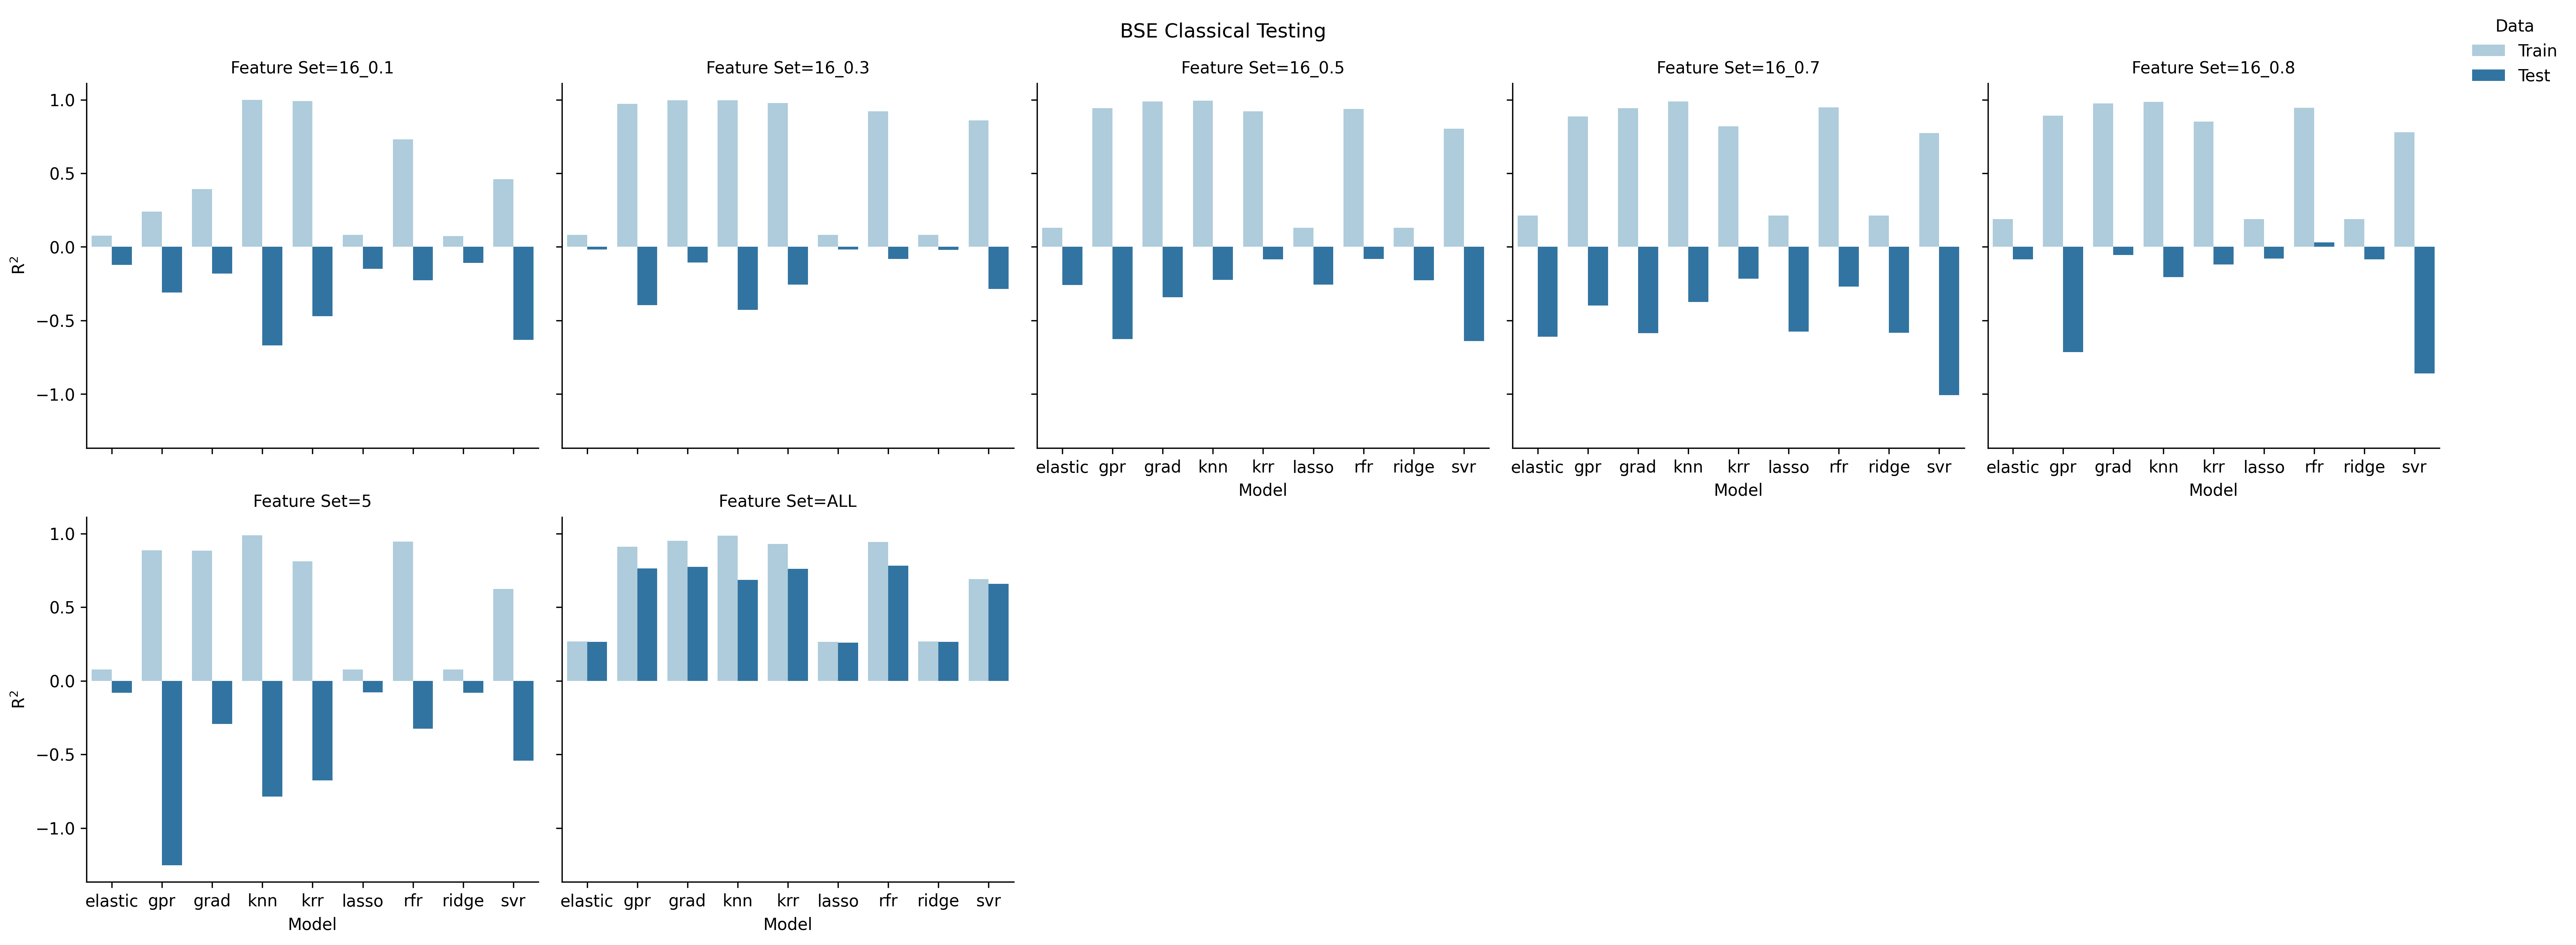
\includegraphics[width=\linewidth]{images/BSE.png}
%	\caption{BSE}
%	\label{fig:BSE}
%\end{figure}


\begin{figure}[H]
	\centering
	\begin{subfigure}[b]{0.3\textwidth}
		\centering
		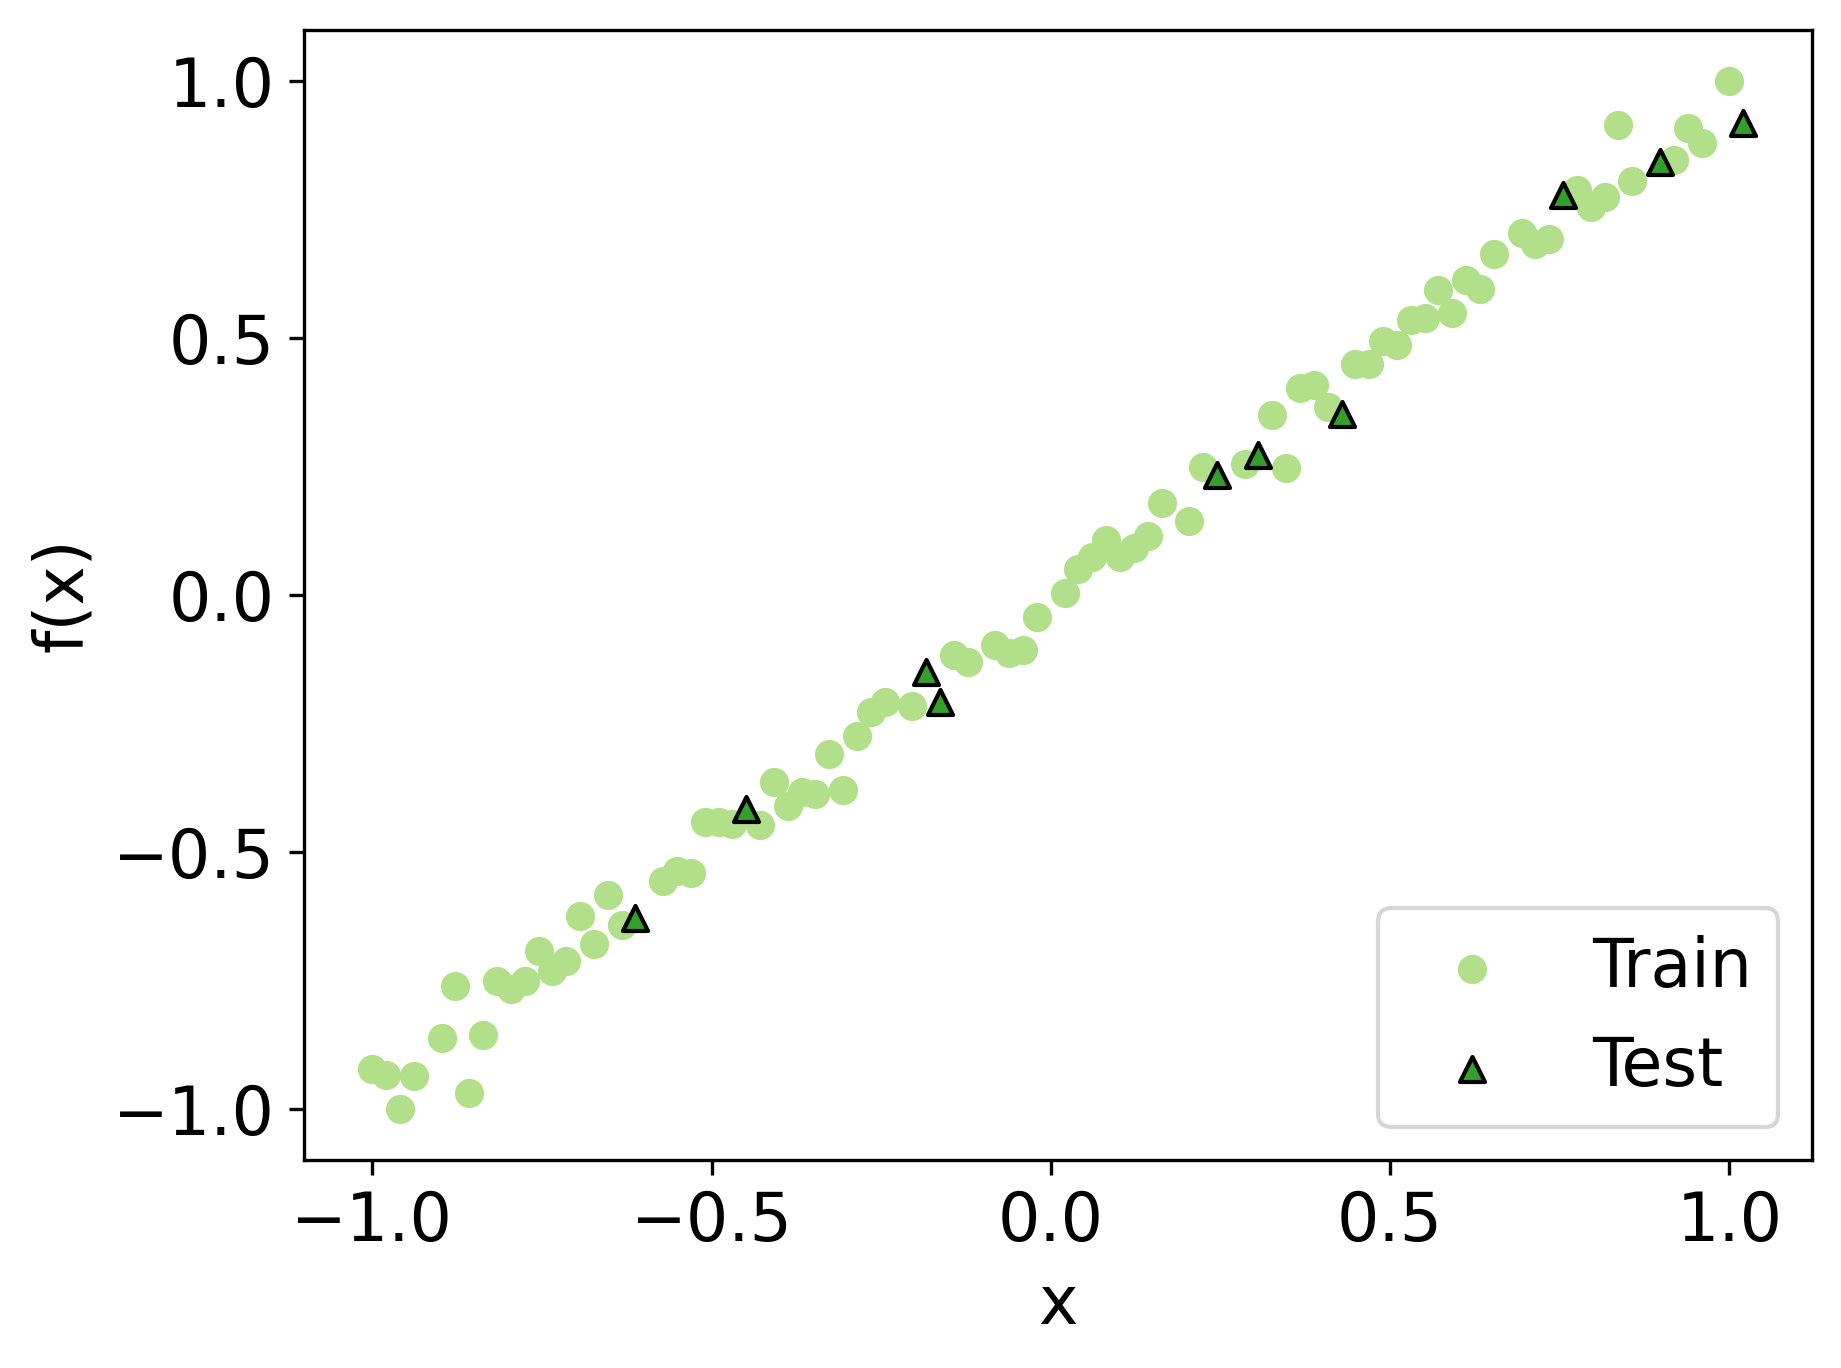
\includegraphics[width=\textwidth]{images/Function_Fitting/function_dataset/linear_train_vs_test.png}
		\caption{}
		\label{fig:linear_train_vs_test}
	\end{subfigure}
	\hfill
	\begin{subfigure}[b]{0.3\textwidth}
		\centering
		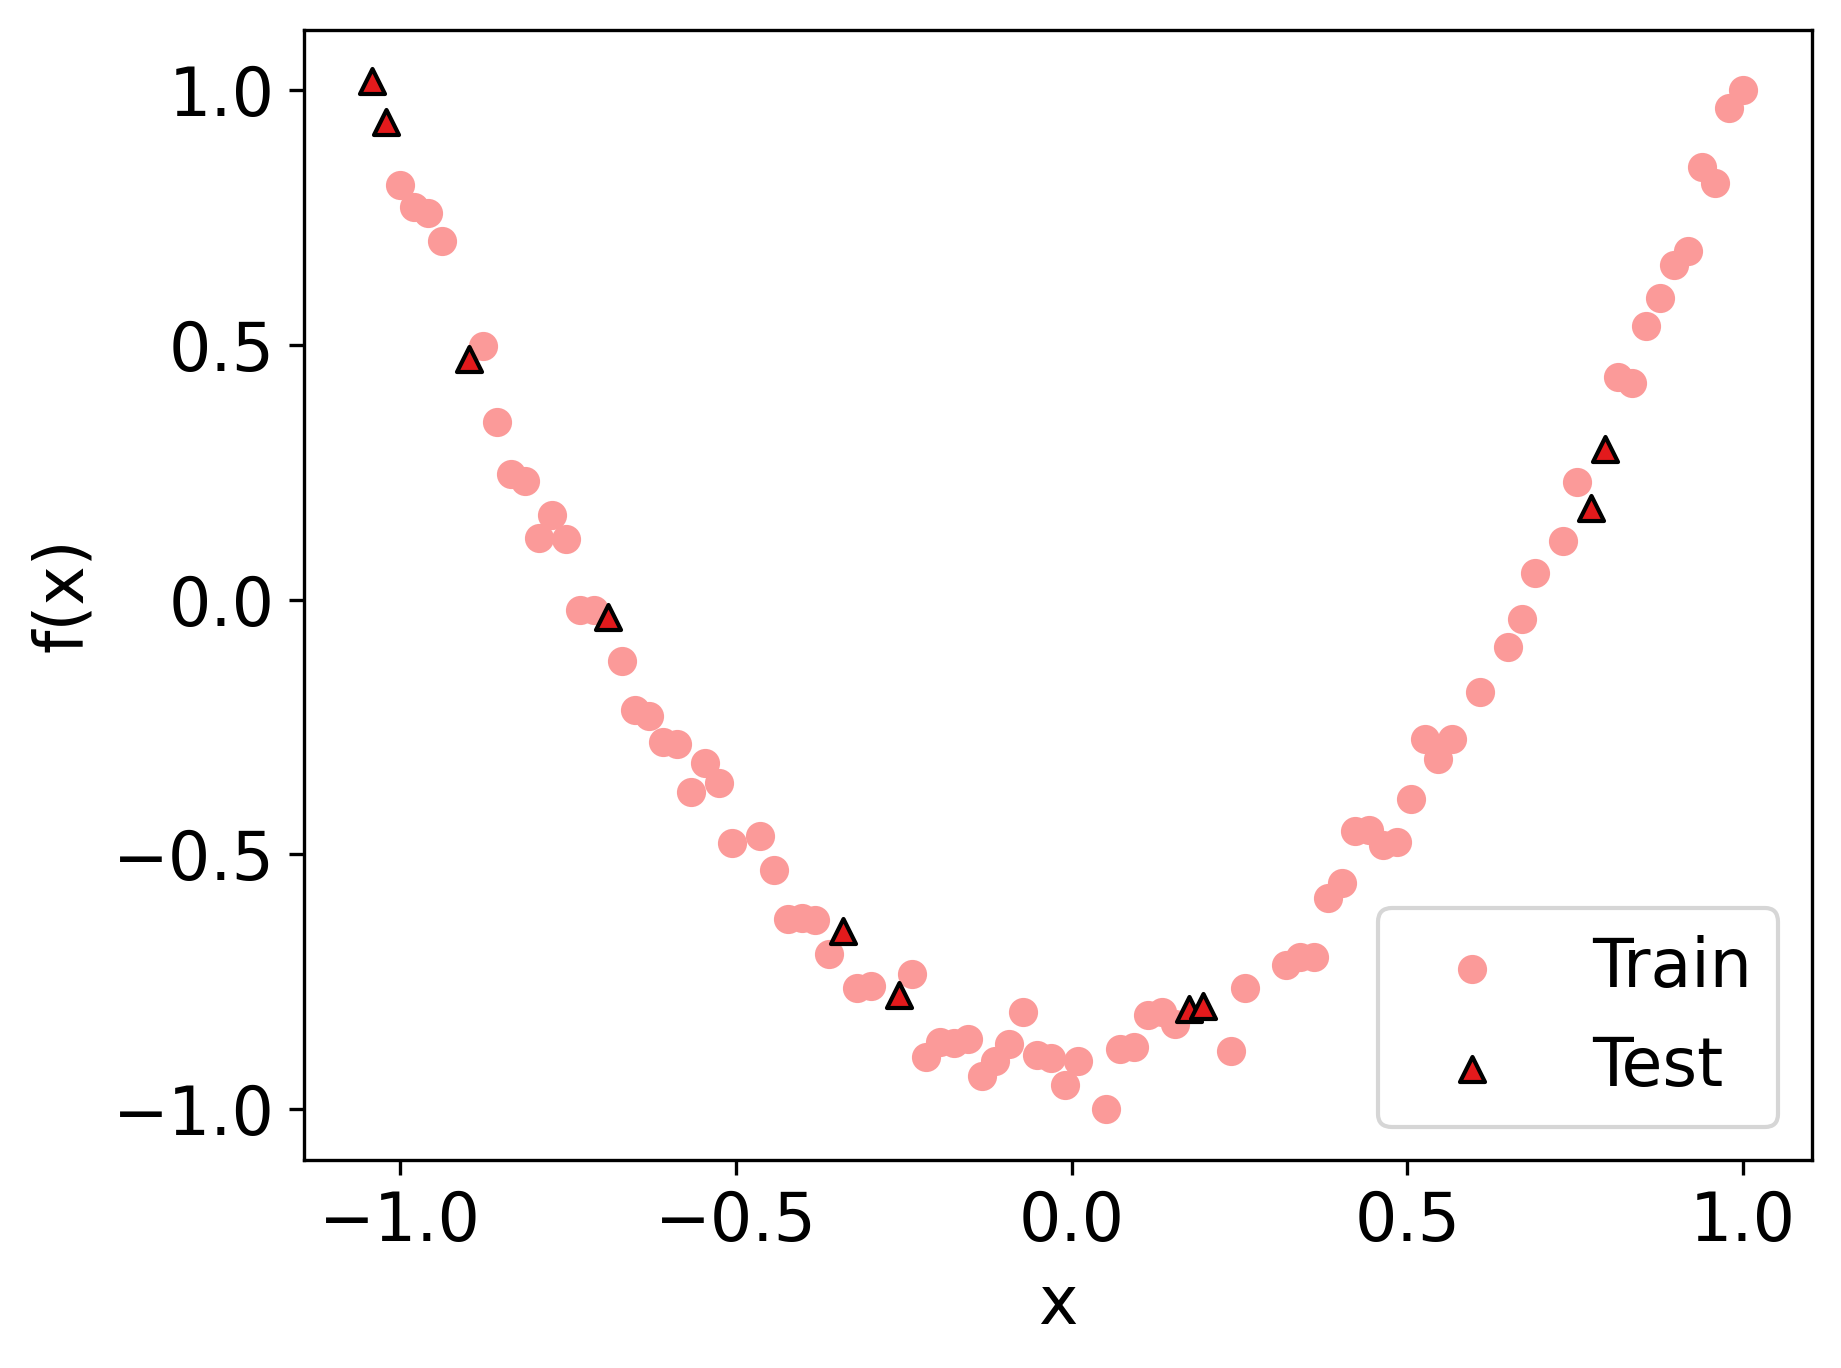
\includegraphics[width=\textwidth]{images/Function_Fitting/function_dataset/quadratic_train_vs_test.png}
		\caption{}
		\label{fig:quadratic_train_vs_test}
	\end{subfigure}
	\hfill
	\begin{subfigure}[b]{0.3\textwidth}
		\centering
		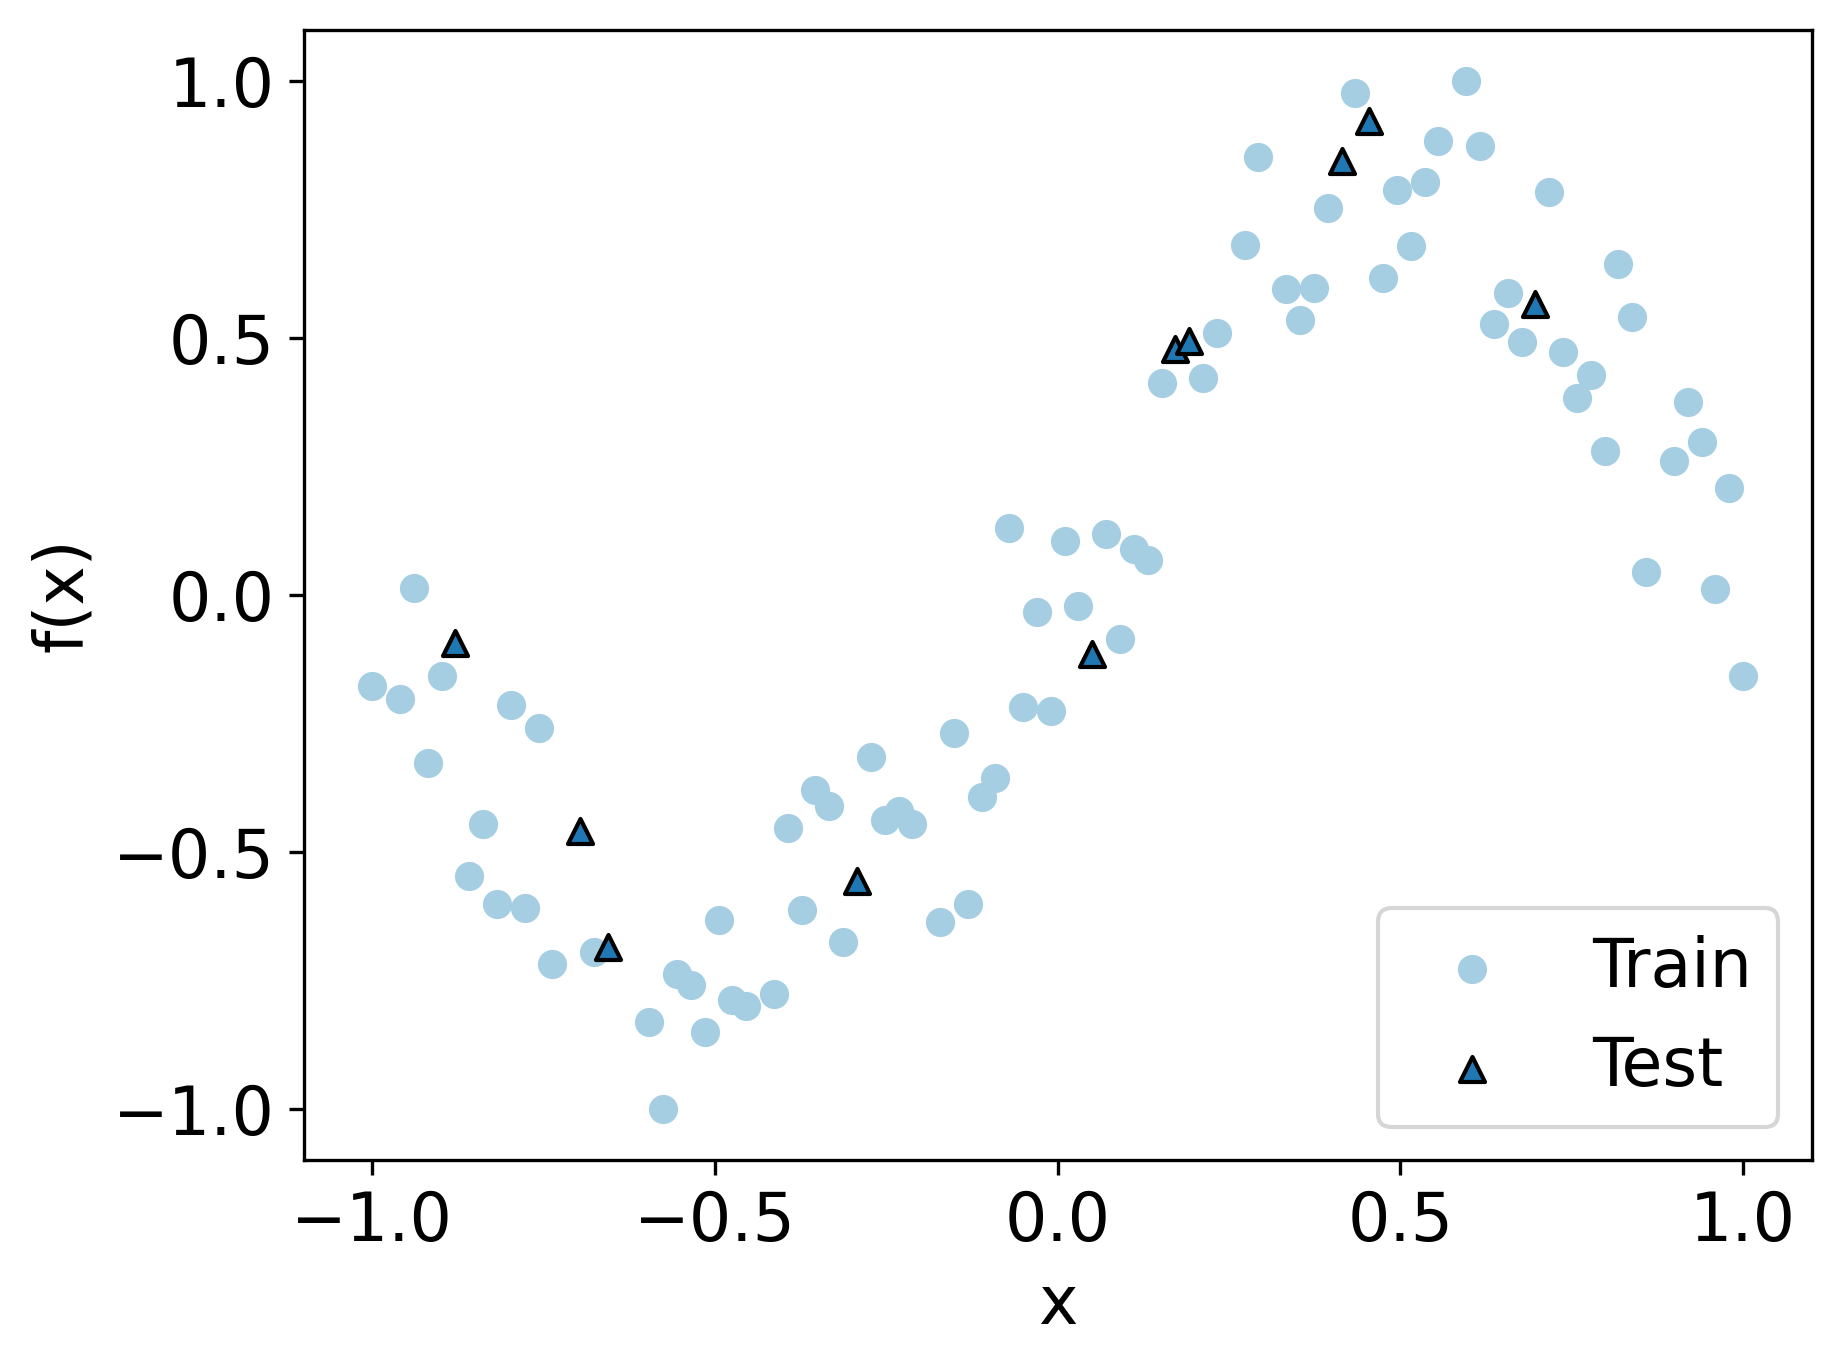
\includegraphics[width=\textwidth]{images/Function_Fitting/function_dataset/sine_train_vs_test.png}
		\caption{}
		\label{fig:sine_train_vs_test}
	\end{subfigure}
	\caption{}
	\label{fig:train_vs_test}
\end{figure}

\section{Results}


Ansaetze analysis \cite{sim_expressibility_2019}
``In particular, a substantial improvement in performance of two-qubit gates in a ring or all-to-all connected arrangement, compared to thatof those on a line, is observed.''

``Furthermore, improvement in both descriptors is achieved by sequences of controlled X-rotation gates compared tosequences of controlled Z-rotation gates.''

``investigated howexpressibility “saturates” with increased circuit depth, finding that the rateand saturated value appear to be distinguishing features of a PQC''



\section{Conclusion}
Depth is not always better!
Molecular representations specifically for QML
Distributed QC to incorporate more features

\bibliography{achemso-demo}

\end{document}
